\chapter{Methodology and validation}

\section{Introduction}
 
A brief overview of the computational methods to perform the simulations to obtain the data in this thesis are are presented in this chapter. As the this particular study is not focused on developing computational methods but concentrated on understanding the physics of a body under the influence of fluid-elastic galloping, it should be noted that the overview provided in this chapter is quite abstract.

The flow of this chapter is as follows. \hilight{First the equations used to model the system are presented and discussed. Next, the a brief discussion of the direct numerical simulation is presented followed by the problem formulation and the discussion of the parameters used.} 

Finally, a series of validation data are presented and discussed to ensure the accuracy of the direct numerical simulations in order to ensure the confidence in the numerical predictions of this thesis.


\subsection{Parameters used}

The data in this project are mainly presented in two categories, high and low Reynolds numbers to compare results at laminar and turbulent range. One main objectives in this study was to capture the flow physics accurately using direct numerical simulations hence,major portion of the study was carried out in the laminar range where the flow is close to 2D. Although majority of data are focused on low Reynolds numbers, some data were presented using inputs from high Reynolds numbers to the QSS model to provide a comparison between high and low Reynolds numbers. $\reynoldsnumber=200$ was defined as the ``low" Reynolds number and $\reynoldsnumber=22300$ was defined as the high Reynolds number. Studies by \citet{tong2008} and \citet{sheard2009} reveals that the approximate value of 3-dimensional transition of the wake for a square cross section is $\reynoldsnumber=160$ and therefore, $\reynoldsnumber=200$ was selected to represent the low Reynolds number regime, also considering the fact that other numerical studies in the laminar regime have used this value for the Reynolds number \citep{Robertson2003,Joly2012}. The reason behind considering the flow regimes of a square cross section was the fact that the basic cross section being used in this study was a square. The selection of the value for the high Reynolds number was fairly was simple as it was the Reynolds number where the pioneering study of galloping \citet{Parkinson1964} provided the experimental input data ($C_y data$) for the QSS model. 

Stationary $C_y$ data at different angles of attack to be used as inputs to the QSS model, were obtained  for the low Reynolds number regime using direct numerical simulations. The average power was obtained by using equation \ref{power}, and the averaging was done over no less than 20 galloping periods. For the high \reynoldsnumber\ tests, predictions of power output at $\reynoldsnumber=22300$ were obtained using the coefficients for the $C_y$  curve from \citet{Parkinson1964}. The mass ratio $m^*$ was kept at 1163 for $\reynoldsnumber=22300$ (Similar to \citet{Parkinson1964}), $m^*=20$ for \reynoldsnumber=200 and $\ustar\geq 40$ similar to the parameters used in literature \citep{Robertson2003,Joly2012} to obtain a comparison with published work. These parameters were used throughout this study unless otherwise specified.

\section{Quasi-steady model}
\label{sec:QSS_model_methodology}

The quasi-steady state model discussed in section \ref{sec:QSS theory} was used to obtain oscillator response data. The quasi-steady state model has proven its ability to obtain accurate galloping response data (discussed in section \ref{sec:QSS theory}). Therefore, it enables to obtain large number of at the expense of a short computational time. The oscillator equation consist of spring, mass and damper oscillator expression with a $7^{th}$ order interpolation polynomial as the forcing function (equation \ref{final_equation_motion}).

\subsubsection{Solving the quasi-steady state equation}

The quasi-steady model being an ordinary differential equation could be solved using different solving methods. Some of the techniques include limit cycle oscillations, harmonic balance, cell mapping and numerical integration. \citet{Vio2007} showed that numerical integration provides accurate data. A fourth-order Runge-Kutta ODE solving scheme was used in solving the quasi-steady state oscillator equation. The built in `ode45' function in MATLAB was used primarily to solve the QSS equation while in some cases `ode15s' function was used when the equation became more stiff.


\section{Calculation of average power}

The ideal potential amount of harvested power output could be represented as the dissipated power due to mechanical damping before losses in any power take-off system are included. Thus the mean power output could be expressed as 


\begin{equation}
\label{eqn:power}
P_{m}=\frac{1}{T}\int_{0}^{T}(c\dot{y})\dot{y} dt,
\end{equation}
where $T$ is the period of integration and $c$ is the mechanical damping constant. 

The work done on the body by the fluid is equal to this quantity, defined as
\begin{equation}
\label{eqn:power_alt}
P_{m}=\frac{1}{T}\int_{0}^{T}F_y\dot{y} dt,
\end{equation}
where $F_y$ is the transverse (lift) force.

The two definitions of the mean power provide two vital interpretations of power transfer. Equation \ref{power} shows that the power is proportional to the mechanical damping and the magnitude of the transverse velocity. At first glance one may assume that the power could be increased by increasing damping. In a practical power extraction device, the significant component of damping would be due to the electrical generator and therefore, an increase in damping would be due to the increase of the load or in other words the electrical resistance. Yet this perception of damping is not quite accurate as very high damping would result in reducing the velocity amplitude which then, would not result in a higher energy output according to equation \ref{power}. In consequence, a balance need to be obtained where the damping is high, but not to the extent that it will adversely result by overly suppressing the motion of the body.  

On the other hand, equation \ref{power_alt} shows that a higher power is attained during situations where the transverse force $F_{y}$ and the transverse velocity are in phase. Hence, a simple increase in the magnitude of the force or the velocity is not satisfactory to attain a higher power transfer. Any increase in magnitude of either of the parameters (force or velocity) is linked to an increase in phase.   



\section{Direct numerical simulations (DNS)}

Direct numerical simulations were employed to obtain the stationary data to be used as inputs to the QSS model and to obtain  fluid-structure interaction (FSI) data to be compared with the QSS model at low Reynolds numbers. A high-order in-house build spectral element which simulates two-dimensional laminar flows was used to obtain the DNS data.


To obtain DNS results an in-house build code was used. This code essentially solves the Naiver-Stokes equations in an accelerated reference frame. A three-step time-splitting scheme also known as a fractional step method was used for temporal discretisation. A predictor-corrector method was used for the FSI data where an elastically mounted body was involved. A description of the spectral element method in general can be found in \citet{karniadakis2005}. This code has been very well validated in a variety of fluid-structure interaction problems similar to that studied in the current study \citep{Leontini2007a,Griffith2011,Leontini2011,Leontini2013}. A overview of the algorithm is presented in the following subsections. 

\subsection{Governing equations}
 
 Assumptions have to be made in any numerical simulation. In this study, the following key assumptions were made to carry out the direct numerical simulations. 
 
 To formulate the differential equations to an infinitesimally small fluid section, the fluid was assumed to be continuum. This assumption is valid for all macro flows. However, it the validity of this assumptions as the fluid dynamics involved reduces to micro and nano scale as the lengths scales involved approaches length scales of the molecules.
 
 Next, To avoid the consideration of acoustic wave propagation it was assumed that the density of the fluid is constant hence, the fluid is incompressible. This particular assumption is valid for Mach numbers (ratio of the speed of sound to the speed of fluid flow ) less than 0.3. In order to disregard the density gradients the fluid was assumed to be isothermal. 
 
 Finally, the fluid was assumed to be an Newtonian fluid, which means that the shear stress is directly proportional to the strain rate. 
 
 These assumptions are quite standard and further information could be found in \citet{White99}.        

The Naiver-Stokes equations are the equations which describes a Newtonian, incompressible contentious fluid.
  \begin{equation} \centering
  \label{eq:nsdim}
  \pderiv{\vecu}{t} + (\vecu\cdot\nabla)\vecu\ = -\frac{\grad{\pres}}{\density} + \frac{\dynvis}{\density}(\gradsq{\vecu})~,
  \end{equation}
  and continuity,
  \begin{equation} \centering
  \divergence{\vecu} = 0~.
  \end{equation}
  
  The velocity vector filed is represented by \vecu, time variable by $t$, the pressure field by \pres \ fluid density by \density \ and the dynamic or kinematic viscosity by \dynvis. In the Naiver-stokes equation (\ref{eq:nsdim}) the left hand side represents the inertial forces and the right hand side represents the pressure forces. The net mass flux into the fluid element is specified to be zero by the continuity equation. 
  
  These equations are generalised by non-dimensionalisation. In the case of bluff body wake flows, the equations are non-dimensionalised by using the characteristic length of the body i.e the frontal projected hight \diam, and the free-stream velocity \Ufree. 
  
  The equations are modified  to  be solved in an accelerated reference frame in this particular study where the frame of reference is attached to the cylinder. Therefore, an extra term is added to the Naiver-stokes equations which the acceleration of the cylinder. Thus, the equations could be written as, 
  
  \begin{equation} \centering
  \label{eq:nsfinal}
  \pderiv{\vecV}{\tau} = -\grad{\Pres} + \frac{1}{\Rey}(\gradsq{\vecV}) - (\vecV\cdot\nabla)\vecV + \accframe ~,
  \end{equation}
  \begin{equation}
  \label{eq:continuity}
  \divergence{\vecV} = 0~.
  \end{equation}
  
   $\vecV = \vecu/U$, $\tau = tU/D$, $\Pres = \pres/(\density
  U^{2})$, $\Rey = \density UD/(\dynvis)$, $\Vcyl = \vcyl/U$, and 
  $\vcyl$ being the velocity of the cylinder. \accframe, represents acceleration term.  
  
  The Naiver-Stokes equations are coupled by with the oscillator differential equation 
  
  \begin{equation} \centering
  \label{eq:cyl_eom}
  \frac{\ddot{y}_{cyl}}{D} + 2\damping\sqrt{\kstar}\frac{\dot{y}_{cyl}}{D} + \kstar\frac{\ycyl}{D} = \frac{\pi}{2}\frac{\clift}{\mstar} ~,
  \end{equation}

  
  
  
    \damping \ is the damping ratio,  $\kstar=kD^{2}/m\Ufree^{2}$ and
    $\clift = \liftf/(0.5\density U^{2}D)$. The lift
    coefficient per unit length of the body is \clift, the transverse displacement of the cylinder is given by \ycyl,  the characteristic length scale of the body is $D$, $k$ is the spring constant and the mass per unit length of the body is represented by $m$. The general form of this linear oscillator equation could be found in books such as  \citet{Naudascher:94}. The final form of the coefficients were constructed by non-dimensionalising the general from of the oscillator equation. 
    
    
 
 \subsection{Temporal discretisation:Time-splitting}
 
 The problem was discretised in order to solve equations \ref{eq:nsfinal}, \ref{eq:continuity} and \ref{eq:cyl_eom} in both space and time. A three-step time splitting method was used for the temporal discretisation. This scheme also known as the fractional step method, was used to separately integrate the terms in the right hand side of the Naiver-Stokes equation. The overall integration of one time-step is split into three substeps. An approximate solution of the Naiver-Stokes equation is gained by this scheme. 
 
 The cylinder acceleration is integrated through the whole time step in order to obtain a initial approximation of the intermediate velocity filed. This velocity filed is used as the stating condition. The pressure is integrated using this starting condition.  A secondary intermediate velocity filed is obtained as a result of the pressure integration substep. This secondary velocity filed is then used as the starting condition for the integration of the diffusion of term which results in the final velocity filed. 
 
 The three semi-discretised substep equations are as follows:
 
\begin{equation} \centering
\label{eq:substep1}
\Vint - \Vn - \Delta\Vcyl = -\int_{\tau}^{\tau+\Delta\tau}(\vecV\cdot\nabla)\vecV \mathrm{d}\tau
\end{equation}
\begin{equation} \centering
\label{eq:substep2}
\Vintint - \Vint = -\int_{\tau}^{\tau+\Delta\tau}\nabla\Pres \mathrm{d}\tau
\end{equation}
\begin{equation} \centering
\label{eq:substep3}
\Vnext-\Vintint = \frac{1}{\Rey}\int_{\tau}^{\tau+\Delta\tau}\gradsq{\vecV} \mathrm{d}\tau,
\end{equation} 
 
The current time step is represented by $n$ and the intermediate velocity fields at the end the convection and pressure substeps are $\Vint$ and $\Vintint$ respectively. The change in the body over a time step is given by $\Delta\Vcyl =
\int_{\tau}^{\tau+\Delta\tau}\accframe \mathrm{d}\tau$. 

The addition of these three substep equations reduces to the integrated form of the Naiver-Stokes equation in equation \ref{eq:nsfinal}. 

\subsubsection{Integration of the substep equations}
\label{subsec:sol}
 
 The integration methods of the pressure, convection and diffusion substeps are presented in this subsection. 
 
 \subsubsection{The convection substep}
 \label{subsub:convec}
 
As the system has a free oscillation, a coupling between the oscillation equation (equation \ref{eq:cyl_eom}) and the Naiver-Stokes equations had to be employed. As a result, the cylinder dynamics had to be solved at each time-step.

An iterative predictor-corrector scheme was scheme was employed to obtain the solution of the coupled equations. The initial step being the ``predictor" step was obtaining approximations for all the quantities involved in  the integration. A quadratic extrapolation was used to obtain an initial estimate of $\Delta\Vcyl$ from  three previous time step values of $\Vcyl$. Therefore, a non-dynamical approximation could be obtained.  
 
 
\begin{equation} \centering
\label{eq:vcyl_start}
\Vcyl^{(n+1)\dag} = 3\Vcyl^{(n)} - 3\Vcyl^{(n-1)} + \Vcyl^{(n-2)} ~,
\end{equation}


The dagger ($\dag$) represents that the value is an initial approximation eg. $\Vcyl^{(n+1)\dag}$. Thus, $\Delta\Vcyl^{\dag}$ was obtained by a simple subtraction of the value at the current time step. 

The approximated position of the cylinder at the next time step could be obtained by carrying out an integration of the cylinder velocity over the time step. A third-order Adams-Moulton method was used to perform the integration. Therefore, the final equation describing the position of the body is given by, 

\begin{equation} \centering
	\label{eq:ycyl_start}
	\frac{\ycyl^{(n+1)\dag} - \ycyl^{(n)}}{\Delta\tau} = \frac{1}{12}(5\Vcyl^{(n+1)\dag} + 8\Vcyl^{(n)} -  
\end{equation}

The transverse displacement of the cylinder is denoted by \ycyl, and the dagger denotes the initial approximation.

An offset is present between the cylinder velocity and cylinder position. The velocity of the cylinder is in advance by half a time-step of the position of the cylinder which is $\Vcyl^{(n+1)}$ is half a time step is in advance of $\ycyl^{(n+1)}$. However, both the cylinder positions and the velocities are located at the same discrete times.

In order to obtain an approximation for \Vint, a solution was obtained for equation \ref{eq:substep1} using the previous approximated quantities.

By using a third-order Adams-Bashforth scheme and incorporating the approximation of equation \ref{eq:vcyl_start} for  $\Delta\Vcyl^{\dag}$ the first approximation for $\Vint$ was obtained using the equation,
 
\begin{equation} \centering
\label{eq:vint_first}
\frac{\Vint - \Vn - \Delta\Vcyl^{\dag}}{\Delta\tau} = \frac{1}{12}(23\mathbf{N}(\vecV)^{(n)} - 16\mathbf{N}(\vecV)^{(n-1)} + 5\mathbf{N}(\vecV)^{(n-2)}) ~.
\end{equation}

The explicit integration method was only used for the first approximation and for the subsequent iterations semi-implicit method was used for $\Vint$.

This step was followed by solving the remaining substep equations in order to obtain an approximation for  $\vecV^{(n+1)\dag}$, and then the ``predictor'' portion of the predictor-corrector method was completed.

The cylinder velocity approximation $\Vcyl^{\dag}$, was updated commencing the ``corrector'' cycle of the predictor-corrector method. This was carried out using a third-order integration scheme. 

 \begin{equation} \centering
 \label{eq:vcyl_correct}
 \frac{\Vcyl^{(n+1)\dag} - \Vcyl^{(n)}}{\Delta\tau} = \frac{1}{24}(25\ddot{y}_{cyl}^{(n+1)} - 2\ddot{y}_{cyl}^{(n)} + \ddot{y}_{cyl}^{(n-1)}) ~.
 \end{equation}
 
 $\Delta\Vcyl^{\dag}$ was updated using the recalculated value of $\Vcyl^{(n+1)\dag}$. The velocity was integrated over a time step in order to obtain the position of the cylinder. For the first correction cycle a third order Adams-Moulton method was used which completed the first iteration of the predictor-corrector method. 
 
 \begin{equation} \centering
 \label{eq:ycyl_correct}
 \frac{y^{(n+1)\dag} - y^{(n)}}{\Delta\tau} = \frac{1}{12}(5\Vcyl^{(n+1)\dag} + 8\Vcyl^{(n)} - \Vcyl^{(n-1)}) ~,
 \end{equation}
 
 Slight modifications were employed to the subsequent iterations in order to improve numerical stability however, the iterations proceeded in a similar manner. As the approximations for  $\Delta\Vcyl^{\dag}$ and $\vecV^{(n+1)\dag}$  were available, using third-order Adams-Moulton scheme further correction steps were employed. 
 
 \begin{equation} \centering
 \label{eq:predict_general}
 \frac{\Vint - \Vn - \Delta\Vcyl^{\dag}}{\Delta\tau} = \frac{1}{12}(5\mathbf{N}(\vecV)^{(n+1)\dag} + 8\mathbf{N}(\vecV)^{(n)} - \mathbf{N}(\vecV)^{(n-1)}) ~.
 \end{equation}
 
 The two remaining substeps were then solved to obtain a new approximation of $\vecV^{(n+1)\dag}$. 
 
 The first correction step was carried out by employing \ref{eq:vcyl_correct} to obtain a second estimate for the velocity of the cylinder $\Vcyl^{(n+1)\ddag}$. A relaxation equation (equation \ref{eq:relax}) was used for the velocity of the cylinder prior to using equation \ref{eq:ycyl_correct} since the equations were quite stiff.
 
 \begin{equation} \centering
 \label{eq:relax}
 \Vcyl^{(n+1)\prime} = \Vcyl^{(n+1)\dag} + \epsilon(\Vcyl^{(n+1)\ddag} - \Vcyl^{(n+1)\dag}) ~,
 \end{equation}
 
 $\Vcyl^{(n+1)\ddag}$ and $\Vcyl^{(n+1)\dag}$ represent the most current and previous approximations respectively. The under relaxation parameter is represented by $\epsilon$ which controls the proportion of the correction which is considered in each iteration. The final approximation at the end of the relaxation process is represented by $\Vcyl^{(n+1)\prime}$ was used in equation \ref{eq:ycyl_correct} in the completing the correction cycle and hence, the iteration.
 
  A convergence error criteria was given until which the iteration was continued. The lift force of the cylinder, the velocity of the cylinder and the fluid velocity should all converge to the required convergence criteria. A series of convergence studies were carried out in order to obtain the convergence criteria \citep{Pregnalato:thesis}. The solution converged within $3-4$ iterations and the iteration count exceeded $10$ in very rare cases.  
  
  The procedure to obtain the solution for $\Vint$ (velocity filed at the end of the convection subsetep) in a nutshell is as follows. A predictor-corrector method was employed, where the primary predictor cycle was first employed. This was followed by obtaining an approximation for $\Delta\Vcyl$ which was calculated using equation \ref{eq:vcyl_start}. From this approximation ($\Delta\Vcyl$)  the position of the cylinder was approximated using equation \ref{eq:ycyl_start}.
 
 Next, using an explicit Adams-Bashforth scheme, an approximation was obtained for $\Vint$ by solving the substep equation (equation \ref{eq:vint_first}). The predictor cycle was completed by solving the remaining substep equations to arrive at the first approximation of \Vnext.   
 
 Then, the primary corrector step was initiated by calculating the forces of the body from the current approximation of \Vnext. Using these forces together with the current approximations of the velocity and the displacement of the body and the equation of motion of the body (eq:\ref{eq:cyl_eom}) an approximation for the acceleration of the cylinder at the end of the timestep was obtained. By integrating this acceleration over the timestep using equation \ref{eq:vcyl_correct} the corrected approximation of $\Delta\Vcyl$ was obtained. Using equation \ref{eq:ycyl_correct} the corrected approximation for $\ycyl^{(n+1)}$  was obtained by integrating the velocity over a timestep by using the recent value of $\Delta\Vcyl$. The primary corrector step and the primary iteration was completed once this step was completed. All the remaining iterations were carried out in a similar manner by with a under relaxation presented in equation \ref{eq:relax}. 
 
 
\subsubsection{The pressure substep}

The pressure equation was solved in two parts in order to find solutions the two unknowns i.e. the pressure filed na d the velocity filed at the end of the timestep. 
 
The integration of the pressure substep was initiated by formulating equation \ref{eq:substep2} in terms of a second-order Adams-Moulton scheme which gives,
 
\begin{equation} \centering
\label{eq:pres_num}
\frac{\Vintint - \Vint}{\Delta\tau} = -\frac{1}{2}(\grad\Pres^{(n+1)} + \grad\Pres^{(n)}) ~.
\end{equation}

The equation was further reduced by considering that the $RHS$ is equal to $\grad\Pres^{(n+1/2)}$. The divergence portion of equation \ref{eq:pres_num} was taken. Using equation \ref{eq:continuity}, continuity was applied to the velocity filed which resulted the pressure filed having a Poisson equation of the form of 

\begin{equation} \centering
\label{eq:poisson}
\gradsq\Pres^{(n+\frac{1}{2})} = \frac{1}{\Delta\tau}\divergence{\Vint} ~.
\end{equation} 

This equation could be solved at the middle of the timestep for the pressure filed. Therefore, this pressure filed could then be back-substituted to equation \ref{eq:pres_num}, together with the simplified $RHS$, to solve for the velocity filed \Vintint, at the end of the substep. 

\subsubsection{The diffusion substep}

A numerical stability of the solution scheme has to be considered for the diffusion substep although the equation for diffusion was linear. Therefore, the Crank-Nicholson scheme or the second order Adams-Moulton scheme which is a semi-implicit scheme which is also unconditionally numerically stable. Thus this formulates the final equation (eq \ref{eq:substep3})of the time splitting scheme as,

\begin{equation} \centering
\label{eq:diff_num}
\frac{\Vnext - \Vintint}{\Delta\tau} = \frac{1}{2\Rey}(\gradsq{\Vnext} + \gradsq{\vecV^{(n)}}) ~.
\end{equation}

The integration over the timestep is completed from the solution of this equation  for \Vnext, thus completing the time splitting scheme. 


\subsubsection{Special discretisation:Spectral element method}
 
 The spacial discretisation was done using a nodal based spectral-element method. This method is a member of the finite-element class. The computational domain is separated into a series of macro elements and then a continuous solution is obtained over each element. Mesh refinement can be done in the areas where high gradients are experienced, which is also known as $h$-refinement. It was necessary that all elements to be quadrilateral. Yet, the elements were not restricted having curved sides.
 
 The calculation of the residual \residual initials the solution process. All the terms of the governing equations (the Naiver-Stokes equation eq \ref{eq:nsfinal}) were moved to the $LHS$. Thus, the resulting expression is, 
 
 \begin{equation} \centering
 \label{eq:ns-oneside}
 \pderiv{\vecV}{\tau} + \grad{\Pres} - \frac{1}{\Rey}(\gradsq{\vecV}) + (\vecV.\nabla)\vecV - \accframe = 0 ~.
 \end{equation}
 
 A trial solution is substituted into the equation \ref{eq:ns-oneside}. The $RHS$ of the equation would be zero if the trial solution is exact solution of the equation. If the trial solution is not the exact solution but an approximation to the exact solution which is the case in general, then the $RHS$ will be non-zero and a residual will be formed. This residual could be defined by, 
 
 \begin{equation} \centering
 \label{eq:residual}
 \pderiv{\Vtrial}{\tau} +\grad{\Ptrial} - \frac{1}{\Rey}(\gradsq{\Vtrial}) + (\Vtrial.\nabla)\Vtrial - \accframe = \residual ~,
 \end{equation}
 
 The trial solutions for velocity and pressure fields are \Vtrial\ and \Ptrial\ respectively. The error term which is introduced through the trial function is the residual \residual. It is clear from equation \ref{eq:residual} that the definition of the residual is the governing equation substituted by the trial solution substituted to the true solution.
 
In order to effectively distribute the error over the domain, the residual has to be weighted in order to minimise the maximum local error. To perform this task the inner product of the residual with a series of weighing functions were taken. The integral of the product of the weighting  function and the residual is the inner product of the residual which is set to zero. The method employed here is also commonly known as weighted residual methods. 

Tensor-product Lagrange polynomials were used for both interpolating trial functions and weighting functions in the DNS carried out in this study. The order of the polynomials $p$ could be varied from $2$ to $14$ in order to further improve grid resolution which is also known as $p$ refinement. This $p$ refinement coupled with $h$ refinement leads to a method called $h-p$ method which is used to improve accuracy \citep{karniadakis2005}. The method also could be referred as a Galerkin method as both trial and weighting functions used were from the same family of functions. \citet{Fletcher84,Fletcher91} provides further details on weighted-residual methods and Galerkin method. 

Lagrange polynomials could be defined as, 

\begin{equation} \centering
\label{eq:lagrange}
L_{i}(\compone) = \underset{g\neq i}{\prod_{g=1}^{p+1}}\frac{(\compone-\compone_{g})}{(\compone_{i}-\compone_{g})}
\end{equation}

The special coordinate is $\compone$ and the indices of the data points are represented by $i$ and $g$ and the number of data points are represented by $p+1$. One of the properties of Lagrange polynomials is that being equal to unity at the point $i$ and being zero at all the other points other than in places in between points. Thus a continuous polynomial which matches the exact values of the velocity at the node point  could be obtained when  $L_{i}$ is multiplied by the velocity at point $i$ and then summing over all points. The tensor-product polynomials in two dimensions $N_{q,s}(\compone, \comptwo)$ could defined as the product of the Lagrange polynomial in one direction $L_{q}(\compone)$, with that in the other direction .$L_{q}(\comptwo)$ 

The outline of the procedure to find the solution is as follows. The process is initiated by forming inner product of the residual and the tensor-product Lagrange polynomial weighting function.

This gives the integral 

 \begin{equation} \centering
 \label{eq:inner-prod}
 \int\int_{\Omega}N_{k,m}(\compone,\comptwo)\cdot[\pderiv{\Vtrial}{\tau} +\grad{\Ptrial} - \frac{1}{\Rey}(\gradsq{\Vtrial}) + (\Vtrial\cdot\nabla)\Vtrial - \accframe]\mathrm{d}x\mathrm{d}y = 0 ~,
 \end{equation}
 
The computational domain is represented by $\Omega$. $N_{q,s}(\compone,\comptwo)$ which are the weighting function is defined in the computational space.

From equation \ref{eq:inner-prod} it is shown that each term in the equation is multiplied by the weighting function. Thus, the integral is split into components and the process could be carried out in the each of the substep equations \ref{eq:substep1}, \ref{eq:substep2} and \ref{eq:substep3}. 


% % % % % % % % % %

The first term in equation \ref{eq:vint_first} could be used as an example to illustrate the process of obtaining the solution using the spectral element method. In order to calculate the integral of the equation (\hilight{use the appropriate equation}) over the entire computational domain, the integral is evaluated over each element separately. After that, the contributions of each element are summed together. 

All the quadrilateral elements are mapped to a square ranging between $-1,1$ in both directions where \compone\ and \comptwo\ are the orthogonal coordinates of this square. The approximation of the integral is simplified by defining the internal node points with the Gauss-Lobatto-Legendre (GLL) quadrature.

A Jacobian is introduced to perform this coordinate transformation and hence, the integral over each element becomes,
\begin{equation} \centering
\label{eq:inner_comp}
\int\int_{El}\Vint N_{q,s}(\compone,\comptwo)\jacobian(\compone, \comptwo)\mathrm{d}\compone \mathrm{d}\comptwo ~,
\end{equation}

The Jacobian is represented by \jacobian and $El$ denotes that the integration is performed over a single element. The solution of equation \ref{eq:inner_comp} $\Vtrial^{*}$, could be re-written as a summation of Lagrange polynomial components. This equation also expresses the tensor-product Lagrange polynomials representing the weighting functions in directions of \compone\ and \comptwo. Therefore, the equation could be expressed as,    

 \begin{equation} \centering
 \label{eq:inner_expand}
 \int\int_{El}\sum_{i,j}\widehat{\Vint}L_{i}(\compone)L_{j}(\comptwo)L_{q}(\compone)L_{s}(\comptwo)\jacobian(\compone, \comptwo)\mathrm{d}\compone \mathrm{d}\comptwo ~.
 \end{equation}
 
 The velocity in the nodal points are represented by $\widehat{\Vint}$, $L$ is the one-dimensional Lagrange polynomial and $i$ and $j$ represents the node locations in directions \compone\ \comptwo. 

The GLL quadrature could be used to obtain an approximation to the integral in equation \ref{eq:inner_expand}, taking the definition of the location of the internal points in the computational domain. Thus approximation of \ref{eq:inner_expand} could be expressed as,

\begin{equation} \centering
\label{eq:inner_GLL}
\sum_{a,b}W_{a,b}\sum_{i,j}\widehat{\Vint}_{i,j}L_{i}(\compone_{a})L_{j}(\comptwo_{b})L_{q}(\compone_{a})L_{s}(\comptwo_{b})\jacobian(\compone_{a}, \comptwo_{b}) ~.
\end{equation}

$W_{a,b}$ represents the weighting coefficient for GLL quadrature, $a$ and $b$ represents the position of the node in the direction \compone\ and \comptwo\ respectively. 


Even though equation \ref{eq:inner_GLL} appears to be quite intimidating to deal with, the expression could be considerably simplified because of the fact that the system is discrete and the only the values at the nodal points are considered. Incorporating Lagrange polynomials allows the substitution 

 \begin{gather}
 \label{eq:kronecker}
 \L_{i}(\compone_{a}) = \delta_{ia} = \begin{cases}
 1 & i = a    \\
 0 & i \neq a \\
 \end{cases} ~.
 \end{gather}
 
 The Kronecker delta is expressed by $\delta_{ia}$. This substitution leads to a significant reduction of the non-zero elements in the simulation and leads to a much simpler expression. If the convection substep (example considered here) is considered, only a single term remains based on \Vint term in the convection substep equation which is,


 \begin{equation} \centering
 W_{q,s}\jacobian(\compone_{q},\comptwo_{s})\widehat{\Vint}_{q,s} ~.
 \end{equation}
 
 
 All the governing terms could be simplified similarly and this process is repeated over all elements. A global matrix is assembled by collecting the contribution of each element and then this matrix system is solved to obtain solution for the unknown velocity and pressure fields at the nodal points. 
 
 Only the continuity of each function is required across the boundaries, with no condition imposed on the gradient (this condition
 is known as $C_{0}$ continuity), even though the shape functions are higher-order polynomials within each element. It can be shown that the method achieves global exponential convergence \citep{karniadakis2005}.  
 
 The numerical process used for this study has been demonstrated to give
 exponential spatial convergence as the number of internal nodes per
 element is increased \citep{Thompson1996a}.
 
 
 
 
 
 
 
 
 
 
 
 




% % % % %



   







\subsubsection{Boundary conditions}

The boundary conditions, regardless of the mesh  were common for all the simulations performed. A no-slip condition was applied to the cross section wall. This condition implied that the velocity is zero at the surface of the cross section. For stationary simulations a Dirichlet boundary condition and for FSI cases a time-dependent Dirichlet boundary condition was employed for the velocity on the inlet and lateral boundaries. A Dirichlet boundary condition should have a specified value for the variables \citep{kreyszig2010} in this case velocity. The time-dependent Dirichlet condition has to be implemented for the FSI cases to account for the accelerated reference frame attached to the cross section. Thus, the inlet boundary was set to $u=U$ and $v=-\dot{y}$ for FSI cases and $v=0$ for stationary cases, where $u,v$ are the velocities in the $x$ and $y$ directions, respectively.

A Neumann condition for the pressure (where the gradient of a property is specified \citet{tu2007}), where the normal gradient was calculated from the Navier--Stokes equations, was employed on the inlet, lateral and body surface \citep{gresho1987}, while a Dirichlet condition for the pressure ($p=0$ was enforced at the outlet. The details of the method can be found in \citet{Thompson2006,Thompson1996a}

 Although the physical validity of the outlet boundary condition is not quite true, this does not turn out to be a significant problem provided that the Reynolds numbers are low and the domain is sufficiently far away from the body.


 
\subsection{Convergence and validation studies}

\subsubsection{Domain size}

 For all cases, a rectangular domain was employed where the inlet was placed $20D$ from the centre of the body, while the outlet was situated $60D$ away from the centre of the body. The lateral boundaries were placed $20D$ away from the centre of the body. The macro element arrangement of the general domain is shown figure \ref{fig:square-mesh} while the element arrangement near the cross sections are presented in figure \ref{fig:zoom-mesh}. 
 
 \begin{figure}[h!]
\setlength{\unitlength}{\textwidth}

  \begin{picture}(0.95,0.5)(0,0.8)
   
  \put(0.2,0.76){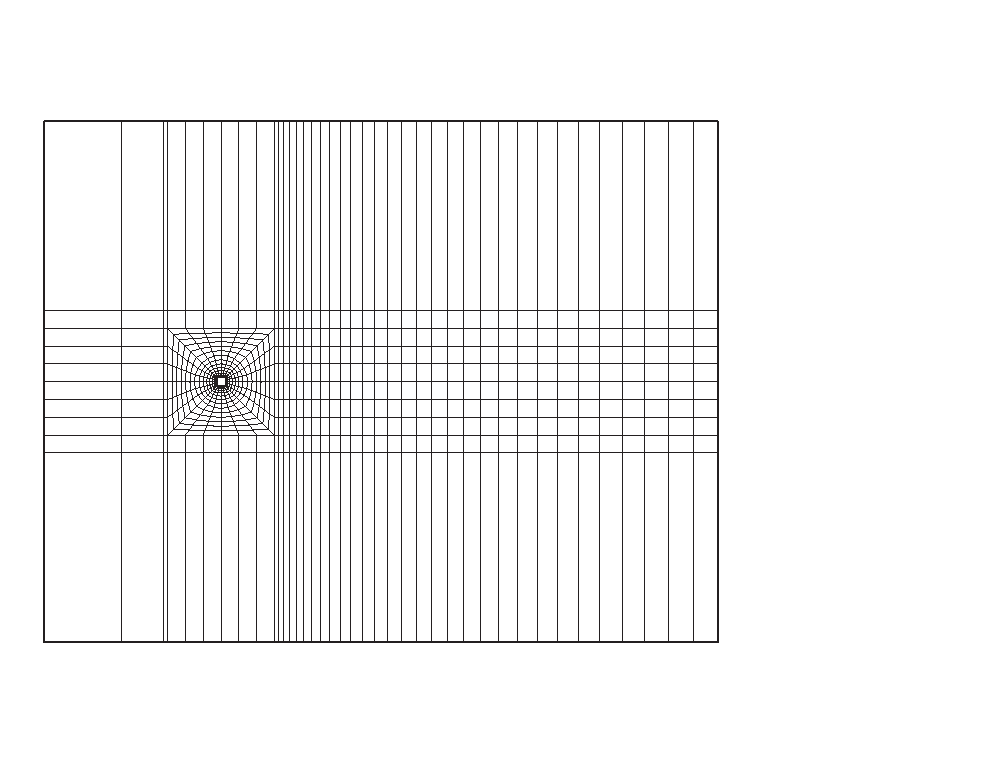
\includegraphics[width=0.8\unitlength]{./chapter-methodology/fnp/square-mesh.eps}}         
      
      
   

      	

  \end{picture}

 \caption{Macro element arrangement in the domain for the square cross section geometry. The inlet extending  $20D$ upstream from the centre of the body, while the outlet extends $60D$ downstream from the centre of the body. The lateral boundaries were placed $20D$ away from the centre of the body.}
    \label{fig:square-mesh}
\end{figure}
 
 
 \begin{figure}
  \setlength{\unitlength}{\textwidth}
\fbox{
  \begin{picture}(0.95,1.3)(0,0.7)
    % % %90
      % % % Parkinson Data 
      \put(0.035,1.65){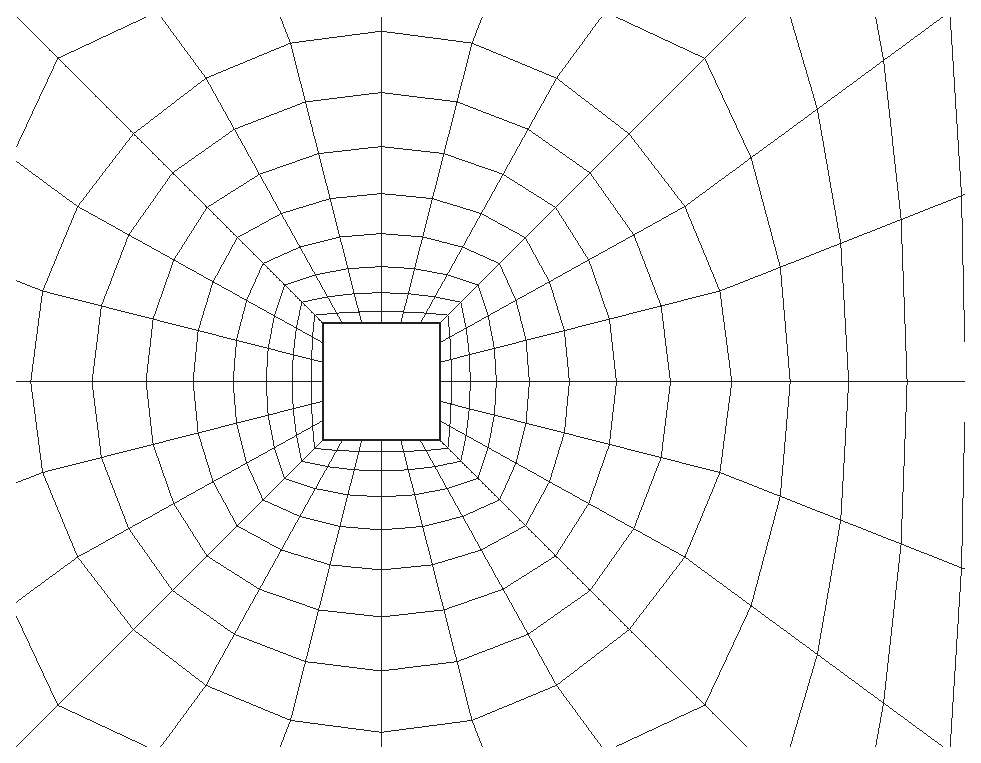
\includegraphics[width=0.4\unitlength]{./chapter-methodology/fnp/mesh.eps}}
      \put(0.495,1.65){\includegraphics[width=0.4\unitlength]{./chapter-methodology/fnp/{hyb0.75-mesh}.eps}}
      \put(0.035,1.25){\includegraphics[width=0.4\unitlength]{./chapter-methodology/fnp/{hyb0.5-mesh}.eps}}
      \put(0.495,1.25){\includegraphics[width=0.4\unitlength]{./chapter-methodology/fnp/{hyb0.25-mesh}.eps}}
      \put(0.3,0.85){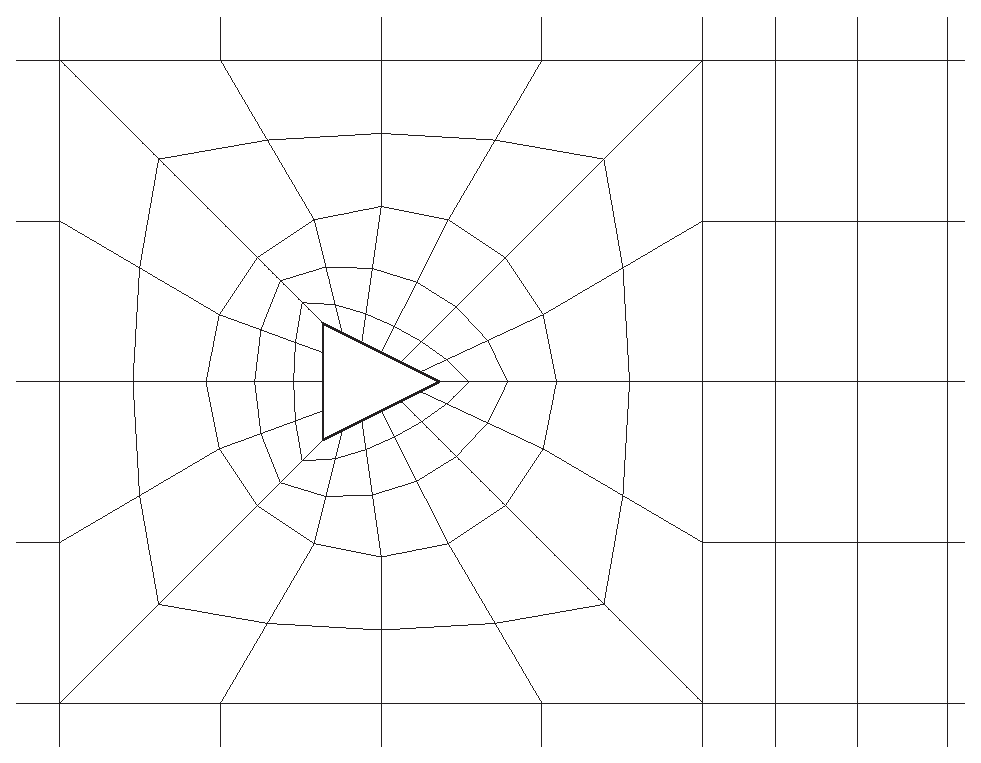
\includegraphics[width=0.4\unitlength]{./chapter-methodology/fnp/triangle-mesh.eps}}
      
      
   
      
      
%      \put(0.23,0.00){ $\displaystyle\frac{c}{\rho\mathcal{A}U}$}
%      \put(0.73,0.00){ $\displaystyle\frac{c}{\rho\mathcal{A}U}$}

     
      \put(0.206,1.605){\small(a)}
      \put(0.665,1.605){\small(b)}
      \put(0.206,1.2){\small(c)}
      \put(0.665,1.2){\small(d)}
      \put(0.45,0.8){\small(e)}
      

  \end{picture}
}
\caption{Configuration of the macro elements near the cross section. (a) square, (b) $\ratio=0.75$, (c) $\ratio=0.5$, (d) $\ratio=0.25$ and (e) triangle.}
  
  \label{fig:zoom-mesh}
\end{figure}

\subsubsection{Convergence}

A series of simulations were carried out in order to ensure the results were grid independent. This was dong by by keeping the layout of the macro element the same and varying the order of the interpolation polynomial (\emph{p-refinement}). The displacement amplitudes were compared against various polynomial orders. The time step was also altered to meet the Courant condition. The summary of the results are presented \hilight{The results table}.


















